\documentclass[11pt]{article} % use larger type; default would be 10pt

\usepackage[utf8]{inputenc} % set input encoding (not needed with XeLaTeX)

\usepackage{geometry} % to change the page dimensions
\geometry{a4paper} % or letterpaper (US) or a5paper or....
% \geometry{margin=2in} % for example, change the margins to 2 inches all round
% \geometry{landscape} % set up the page for landscape
%   read geometry.pdf for detailed page layout information

\usepackage{graphicx} % support the \includegraphics command and options
\usepackage{authblk}
\usepackage{url}

% \usepackage[parfill]{parskip} % Activate to begin paragraphs with an empty line rather than an indent

%%% PACKAGES
\usepackage{booktabs} % for much better looking tables
\usepackage{array} % for better arrays (eg matrices) in maths
\usepackage{paralist} % very flexible & customisable lists (eg. enumerate/itemize, etc.)
\usepackage{verbatim} % adds environment for commenting out blocks of text & for better verbatim
\usepackage{subfig} % make it possible to include more than one captioned figure/table in a single float
% These packages are all incorporated in the memoir class to one degree or another...

\usepackage[polish]{babel}	
\usepackage{polski}
\usepackage[T1]{fontenc}
\frenchspacing	

\usepackage{indentfirst}

\usepackage{fancyhdr} % This should be set AFTER setting up the page geometry
\pagestyle{fancy} % options: empty , plain , fancy
\renewcommand{\headrulewidth}{0pt} % customise the layout...
\lhead{}\chead{}\rhead{}
\lfoot{}\cfoot{\thepage}\rfoot{}

%%% SECTION TITLE APPEARANCE
\usepackage{sectsty}
\allsectionsfont{\sffamily\mdseries\upshape} % (See the fntguide.pdf for font help)
% (This matches ConTeXt defaults)

%%% ToC (table of contents) APPEARANCE
\usepackage[nottoc,notlof,notlot]{tocbibind} % Put the bibliography in the ToC
\usepackage[titles,subfigure]{tocloft} % Alter the style of the Table of Contents
\renewcommand{\cftsecfont}{\rmfamily\mdseries\upshape}
\renewcommand{\cftsecpagefont}{\rmfamily\mdseries\upshape} % No bold!

%%% END Article customizations

%%% The "real" document content comes below...

\title{San Francisco Crime Classification\\ \large{Kaggle competition  }}
\author{Łukasz Rados, Wojciech Kusa}

\affil{Wydział Fizyki i Informatyki Stosowanej \\ Akademia Górniczo-Hutnicza w Krakowie}


%\date{} % Activate to display a given date or no date (if empty),
         % otherwise the current date is printed 

\begin{document}
\maketitle

\section{Wprowadzenie}

Celem projektu było stworzenie oprogramowania pozwalającego dokonać klasyfikacji przestępstw na podstawie danych czasoprzestrzennych z raportów policyjnych dla miasta San Francisco w Stanach Zjednoczonych. Pełen opis projektu, wraz z danymi wejściowymi znajduje się na portalu kaggle, pod adresem: \url{www.kaggle.com/c/sf-crime/}.


\section{Dane} \label{sec:data}

Zbiór danych zawiera incydenty zgłoszone policji w San Francisco pomiędzy 01.01.2003r. a 13.05.2015r.. Podzielony jest na dwie podgrupy (prawie równoliczne, w każdej po około 850 tysięcy elementów) :
\begin{itemize}
\item zbiór treningowy -- zawierający zgłoszenia z tygodni parzystych,

\item zbiór testowy --  zawierający zgłoszenia z tygodni nieparzystych.
\end{itemize} 

Przykładowe wiersze danych treningowych znajdują się na Rysunku \ref{fig:train_data}. Dane składają się z następujących pól:

\begin{itemize}
\item Dates -- znacznik czasu przestępstwa
\item DayOfWeek -- dzień tygodnia
\item PdDistrict -- nazwa departamentu policji odbierającego zgłoszenie
\item Address -- przybliżony adres przestępstwa
\item X -- długość geograficzna
\item Y -- szerokość geograficzna
\item Category -- kategoria przestępstwa (tylko dla zbioru treingowego). Jest to zmienna, którą należało przewidzieć w wyniku działania algorytmu
\item Descript -- szczegółowy opis przestępstwa (tylko dla zbioru treingowego)
\item Resolution -- jaki był wynik działania policji (tylko dla zbioru treingowego)

\end{itemize}

\begin{figure}[!h]
  \centering
    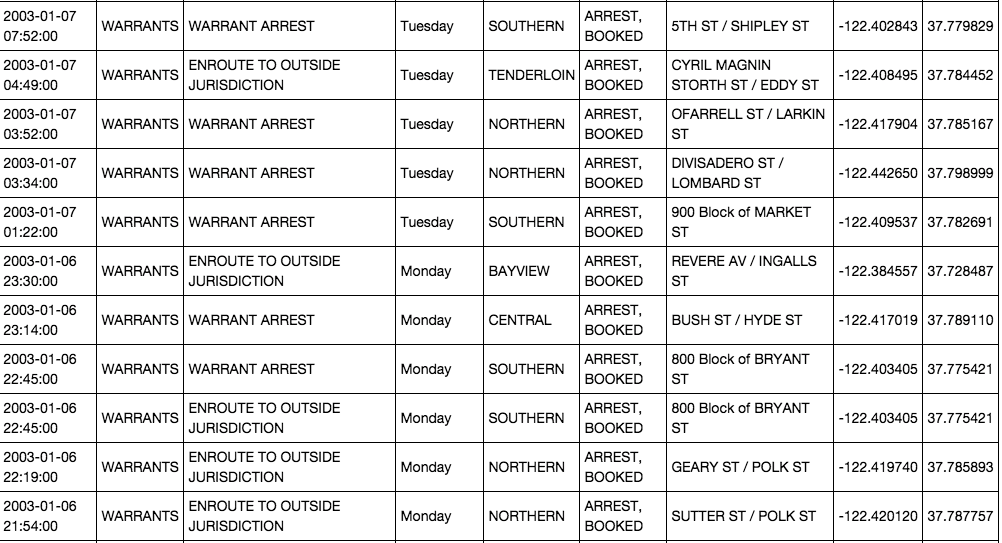
\includegraphics[width=0.95\textwidth]{images/train_data.png}
  \caption{Przykładowe dane treningowe. Źródło: \protect\url{https://www.kaggle.com/c/sf-crime/data} } \label{fig:train_data}
\end{figure}



\subsection{Wstępna analiza zbioru treningowego}

Na rysunku \ref{fig:sf_districts} znajduje się mapa San Francisco z zaznaczpnymi wszystkimi przestępstami podzielonymi ze względu na posterunek odbierający zgłoszenie.


\begin{figure}[!h]
  \centering
    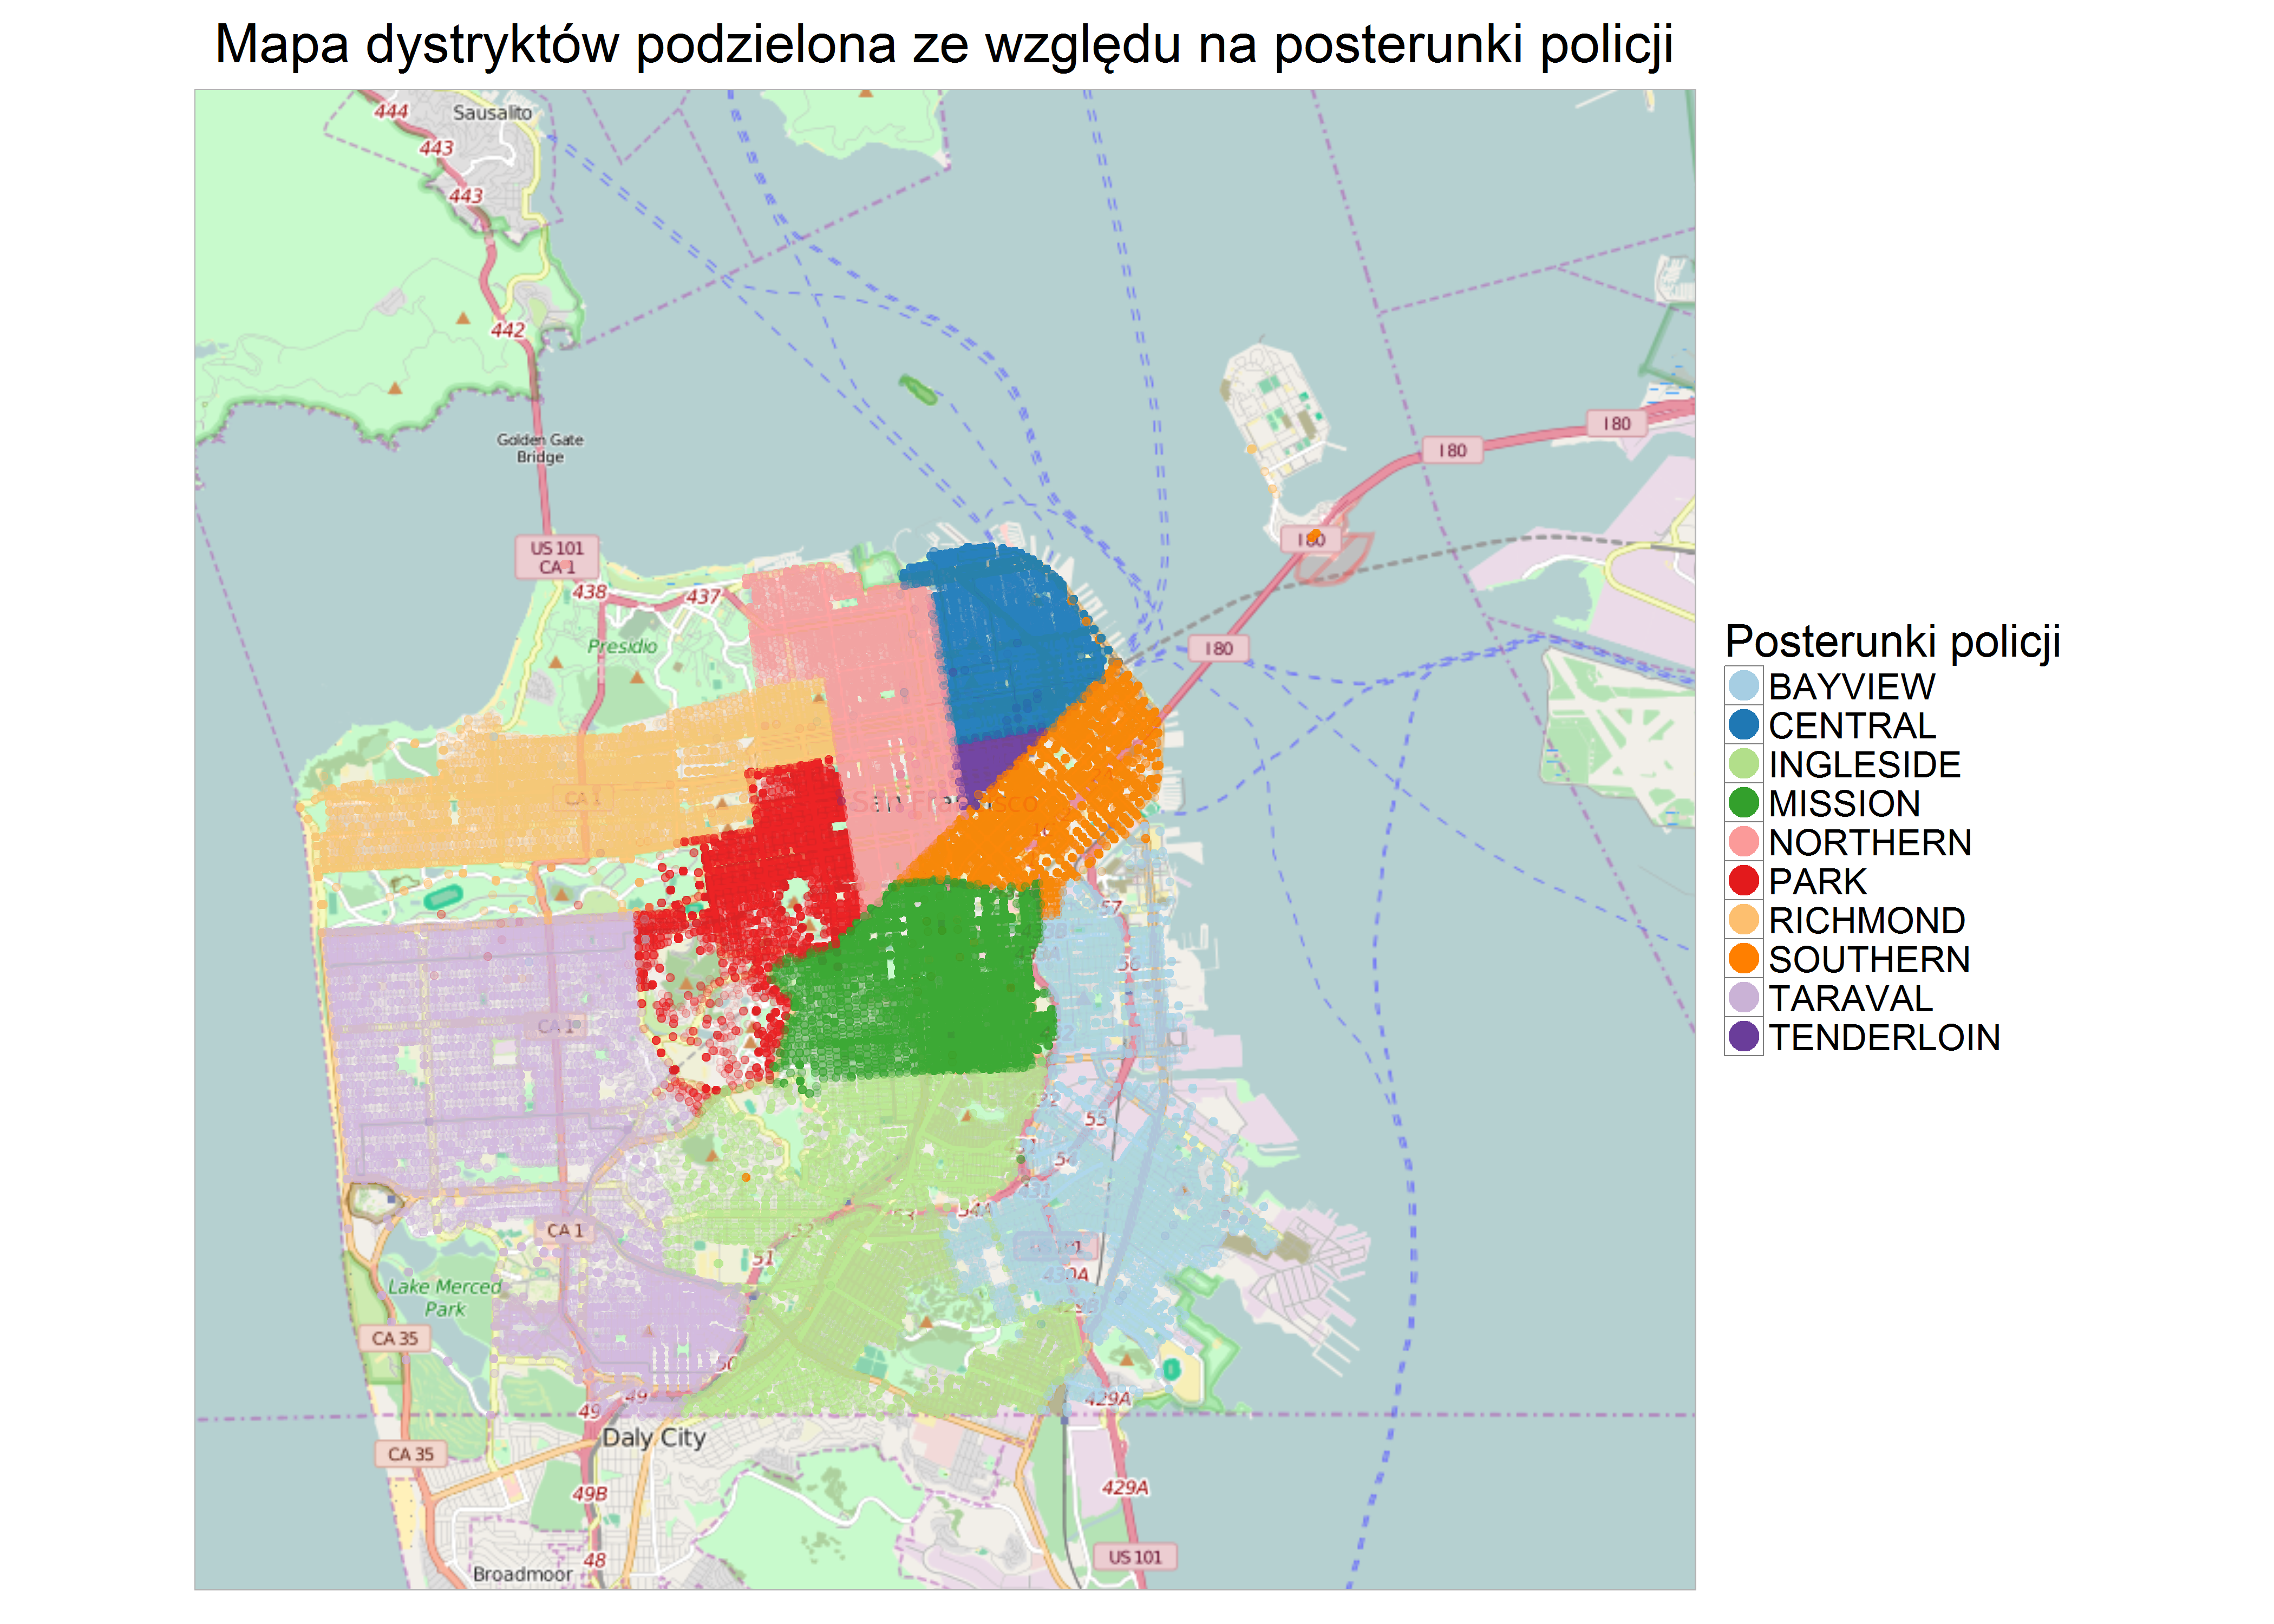
\includegraphics[width=0.95\textwidth]{images/sf_districts}
  \caption{Przestępstwa podzielone ze względu na posterunek odbierający zgłoszenie.} \label{fig:sf_districts}
\end{figure}


\subsection{Zastosowane deskryptory}

Dane poddane zostały preprocessingowi celem poprawy brakujących rekordów, a następnie, poza podstawowymi zmiennymi przedstawionymi w sekcji \ref{sec:data}, przygotowano dodatkowe deskryptory mające pomóc wytrenować model. Poniżej zostały opisane najważniejsze z nich, mające istotny wpływ na poprawę działania modelu:

\begin{itemize}
\item $Dates.Hours \cdot 60 + Dates.Minutes$ - Liczba z zakreu {0, 1440} opisująca, w której minucie dnia zostało dokonane zgłoszenie

\item $X \cdot Y$ - wskazuje na nieliniową korelację długości i szerokości geograficznej

\item $X + Y$ - jak wyżej, zmienna wskazująca na korelację długości i szerokości geograficznej

\item informacja czy przestępstwo zostało dokonane na skrzyżowaniu / rogu ulicy - wyciągnięta ze zmiennej Address

\item informacja czy przestępstwo zostało dokonane w bloku - wyciągnięta ze zmiennej Address

\item $DayOfWeek + Dates.Hour$  - powiązuje godzinę zdarzenia z dniem tygodnia

\item $DayOfWeek \cdot Dates.Hour$ -  jak wyżej, powiązuje godzinę zdarzenia z dniem tygodnia

\end{itemize}


\section{Zastosowane algorytmy}
\subsection{Lasy losowe - Random Forest}

\subsection{Generalized Linear Model}


\section{Implementacja}

Kody źródłowe zaimplementowanych modeli znajdują się w repozytorium on-line pod adresem \url{www.github.com/WojciechKusa/sf_crime}. \\

Model wykorzystujący GLM zaimplementowany został w języku R z wykorzystaniem bibliotek MASS, readr, rpart oraz caret. Do ostatecznego modelu wzięte zostały następujące zmienne:

\begin{itemize}
\item $PdDistrict$

\item $X $
\item $Y $
\item $X \cdot Y$
\item $X + Y$ 
\item $DayOfWeek$
\item $Dates.Year $
\item $Dates.Month $
\item $Dates.Hour $
\item $Dates.Hours \cdot 60 + Dates.Minutes$ 
\item $DayOfWeek + Dates.Hour $
\item $DayOfWeek \cdot Dates.Hour $

\item $AddType $

\end{itemize}



\section{Ewaluacja oraz wyniki}

\subsection{Ocena modeli}

Ocena modeli dokonywana była na podstawie wielo-klasowej straty logarytmicznej (ang. \textit{multi-class logarithmic loss}). Dane zawierały prawdopodobieństwa wystąpienia danego przestępstwa przy podanych danych czasoprzestrzennych. \\

\subsection{Uzyskane wyniki}


W przypadku zastosowania modelu GLM uzyskany wynik to 2.54389 punkta co na dzień 24.01.2016r. dało 314 miejsce na 1200 uczestników. Dla modelu RF otrzymano wynik 5.70246 co plasuje go na 889 miejscu. Wyniki te można uznać za satysfakcjonując gdy weźmie się pod uwagę fakt, że najlepszy aktualnie wynik to 2.05079 a pierwsze 900 rezultatów to wyniki poniżej 10 punktów.\\


\section{Podsumowanie}



\end{document}
